\documentclass{report}
\usepackage[english]{babel}

%%%%%%%%%%%%%%%%%%%%%%%%%%%%%%%%%
% PACKAGE IMPORTS
%%%%%%%%%%%%%%%%%%%%%%%%%%%%%%%%%


\usepackage[tmargin=2cm,rmargin=1in,lmargin=1in,margin=0.85in,bmargin=2cm,footskip=.2in]{geometry}
\usepackage{amsmath,amsfonts,amsthm,amssymb,mathtools}
\usepackage{wrapfig}
\usepackage{subcaption}
\usepackage{afterpage}
\usepackage[varbb]{newpxmath}
\usepackage{xfrac}
\usepackage[T1]{fontenc}
\usepackage{tabularx}
\usepackage{floatrow}
\usepackage{enumerate}
\newfloatcommand{capbtabbox}{table}[][\FBwidth]
\usepackage{amssymb}
%command for alg-closure that automatically adapts its 'bar' to the arg based on the args length (including '\')
\newcommand{\ols}[1]{\mskip.5\thinmuskip\overline{\mskip-.5\thinmuskip {#1} \mskip-.5\thinmuskip}\mskip.5\thinmuskip} % overline short
\newcommand{\olsi}[1]{\,\overline{\!{#1}}} % overline short italic
\makeatletter
\newcommand\ovl[1]{
  \tctestifnum{\count@stringtoks{#1}>1} %checks if number of chars in arg > 1 (including '\')
  {\ols{#1}} %if arg is longer than just one char, e.g. \mathbb{Q}, \mathbb{F},...
  {\olsi{#1}} %if arg is just one char, e.g. K, L,...
}
% FROM TOKCYCLE:
\long\def\count@stringtoks#1{\tc@earg\count@toks{\string#1}}
\long\def\count@toks#1{\the\numexpr-1\count@@toks#1.\tc@endcnt}
\long\def\count@@toks#1#2\tc@endcnt{+1\tc@ifempty{#2}{\relax}{\count@@toks#2\tc@endcnt}}
\def\tc@ifempty#1{\tc@testxifx{\expandafter\relax\detokenize{#1}\relax}}
\long\def\tc@earg#1#2{\expandafter#1\expandafter{#2}}
\long\def\tctestifnum#1{\tctestifcon{\ifnum#1\relax}}
\long\def\tctestifcon#1{#1\expandafter\tc@exfirst\else\expandafter\tc@exsecond\fi}
\long\def\tc@testxifx{\tc@earg\tctestifx}
\long\def\tctestifx#1{\tctestifcon{\ifx#1}}
\long\def\tc@exfirst#1#2{#1}
\long\def\tc@exsecond#1#2{#2}
\makeatother
\usepackage[makeroom]{cancel}
\usepackage{mathtools}
\usepackage{bookmark}
\usepackage{enumitem}
\usepackage{hyperref,theoremref}
\hypersetup{
	pdftitle={Apuntes de Análisis de Varias Variables 2},
	colorlinks=true, linkcolor=doc!90,
	bookmarksnumbered=true,
	bookmarksopen=true
}
\usepackage[most,many,breakable]{tcolorbox}
\usepackage{xcolor}
\usepackage{varwidth}
\usepackage{varwidth}
\usepackage{etoolbox}
%\usepackage{authblk}
\usepackage{nameref}
\usepackage{multicol,array}
\usepackage{tikz-cd}
\usepackage[ruled,vlined,linesnumbered]{algorithm2e}
\usepackage{comment} % enables the use of multi-line comments (\ifx \fi) 
\usepackage{import}
\usepackage{xifthen}
\usepackage{pdfpages}
\usepackage{transparent}
\usepackage{titlesec}
\titleformat{\section}{\normalfont\fontsize{17.28pt}{12pt}\selectfont\bfseries}{\thesection}{1em}{}
\usepackage{empheq} % boxed align


\newcommand\mycommfont[1]{\footnotesize\ttfamily\textcolor{blue}{#1}}
\SetCommentSty{mycommfont}
\newcommand{\incfig}[1]{%
    \def\svgwidth{\columnwidth}
    \import{./figures/}{#1.pdf_tex}
}

\newcommand{\notimplies}{\;\not\!\!\!\implies}

\usepackage{tikzsymbols}
\renewcommand\qedsymbol{$\Laughey$}

\newcommand\phantomarrow[2]{%
  \setbox0=\hbox{$\displaystyle #1\to$}%
  \hbox to \wd0{%
    $#2\mapstochar
     \cleaders\hbox{$\mkern-1mu\relbar\mkern-3mu$}\hfill
     \mkern-7mu\rightarrow$}%
  \,}

%\usepackage{import}
%\usepackage{xifthen}
%\usepackage{pdfpages}
%\usepackage{transparent}


%%%%%%%%%%%%%%%%%%%%%%%%%%%%%%
% SELF MADE COLORS
%%%%%%%%%%%%%%%%%%%%%%%%%%%%%%



\definecolor{myg}{RGB}{56, 140, 70}
\definecolor{myb}{RGB}{45, 111, 177}
\definecolor{myr}{RGB}{199, 68, 64}
\definecolor{mytheorembg}{HTML}{f5e4e1}
\definecolor{mytheoremfr}{HTML}{7B0000}
\definecolor{mylenmabg}{HTML}{FFFAF8}
\definecolor{mylenmafr}{HTML}{983b0f}
\definecolor{mypropbg}{HTML}{f2fbfc}
\definecolor{mypropfr}{HTML}{191971}
\definecolor{myexamplebg}{HTML}{F2FBF8}
\definecolor{myexamplefr}{HTML}{88D6D1}
\definecolor{myexampleti}{HTML}{2A7F7F}
\definecolor{mydefinitbg}{HTML}{E5E5FF}
\definecolor{mydefinitfr}{HTML}{3F3FA3}
\definecolor{notesgreen}{RGB}{0,162,0}
\definecolor{myp}{RGB}{197, 92, 212}
\definecolor{mygr}{HTML}{2C3338}
\definecolor{myred}{RGB}{127,0,0}
\definecolor{myyellow}{RGB}{169,121,69}
\definecolor{myexercisebg}{HTML}{F2FBF8}
\definecolor{myexercisefg}{HTML}{2A7F7F}


%%%%%%%%%%%%%%%%%%%%%%%%%%%%
% TCOLORBOX SETUPS
%%%%%%%%%%%%%%%%%%%%%%%%%%%%

\setlength{\parindent}{1cm}
%================================
% THEOREM BOX
%================================

\tcbuselibrary{theorems,skins,hooks}
\newtcbtheorem[number within=section]{Theorem}{Teorema}
{%
	enhanced,
	breakable,
	colback = mytheorembg,
	frame hidden,
	boxrule = 0sp,
	borderline west = {2pt}{0pt}{mytheoremfr},
	sharp corners,
	detach title,
	before upper = \tcbtitle\par\smallskip,
	coltitle = mytheoremfr,
	fonttitle = \bfseries\sffamily,
	description font = \mdseries,
	separator sign none,
	segmentation style={solid, mytheoremfr},
}
{th}

\tcbuselibrary{theorems,skins,hooks}
\newtcbtheorem[number within=chapter]{theorem}{Teorema}
{%
	enhanced,
	breakable,
	colback = mytheorembg,
	frame hidden,
	boxrule = 0sp,
	borderline west = {2pt}{0pt}{mytheoremfr},
	sharp corners,
	detach title,
	before upper = \tcbtitle\par\smallskip,
	coltitle = mytheoremfr,
	fonttitle = \bfseries\sffamily,
	description font = \mdseries,
	separator sign none,
	segmentation style={solid, mytheoremfr},
}
{th}


\tcbuselibrary{theorems,skins,hooks}
\newtcolorbox{Theoremcon}
{%
	enhanced
	,breakable
	,colback = mytheorembg
	,frame hidden
	,boxrule = 0sp
	,borderline west = {2pt}{0pt}{mytheoremfr}
	,sharp corners
	,description font = \mdseries
	,separator sign none
}

%================================
% Corollary
%================================
\tcbuselibrary{theorems,skins,hooks}
\newtcbtheorem[number within=section]{Corollary}{Corolario}
{%
	enhanced
	,breakable
	,colback = myp!10
	,frame hidden
	,boxrule = 0sp
	,borderline west = {2pt}{0pt}{myp!85!black}
	,sharp corners
	,detach title
	,before upper = \tcbtitle\par\smallskip
	,coltitle = myp!85!black
	,fonttitle = \bfseries\sffamily
	,description font = \mdseries
	,separator sign none
	,segmentation style={solid, myp!85!black}
}
{th}
\tcbuselibrary{theorems,skins,hooks}
\newtcbtheorem[number within=chapter]{corollary}{Corolario}
{%
	enhanced
	,breakable
	,colback = myp!10
	,frame hidden
	,boxrule = 0sp
	,borderline west = {2pt}{0pt}{myp!85!black}
	,sharp corners
	,detach title
	,before upper = \tcbtitle\par\smallskip
	,coltitle = myp!85!black
	,fonttitle = \bfseries\sffamily
	,description font = \mdseries
	,separator sign none
	,segmentation style={solid, myp!85!black}
}
{th}


%================================
% LENMA
%================================

\tcbuselibrary{theorems,skins,hooks}
\newtcbtheorem[number within=section]{Lenma}{Lenma}
{%
	enhanced,
	breakable,
	colback = mylenmabg,
	frame hidden,
	boxrule = 0sp,
	borderline west = {2pt}{0pt}{mylenmafr},
	sharp corners,
	detach title,
	before upper = \tcbtitle\par\smallskip,
	coltitle = mylenmafr,
	fonttitle = \bfseries\sffamily,
	description font = \mdseries,
	separator sign none,
	segmentation style={solid, mylenmafr},
}
{th}

\tcbuselibrary{theorems,skins,hooks}
\newtcbtheorem[number within=chapter]{lenma}{Lenma}
{%
	enhanced,
	breakable,
	colback = mylenmabg,
	frame hidden,
	boxrule = 0sp,
	borderline west = {2pt}{0pt}{mylenmafr},
	sharp corners,
	detach title,
	before upper = \tcbtitle\par\smallskip,
	coltitle = mylenmafr,
	fonttitle = \bfseries\sffamily,
	description font = \mdseries,
	separator sign none,
	segmentation style={solid, mylenmafr},
}
{th}


%================================
% PROPOSITION
%================================

\tcbuselibrary{theorems,skins,hooks}
\newtcbtheorem[number within=section]{Prop}{Proposition}
{%
	enhanced,
	breakable,
	colback = mypropbg,
	frame hidden,
	boxrule = 0sp,
	borderline west = {2pt}{0pt}{mypropfr},
	sharp corners,
	detach title,
	before upper = \tcbtitle\par\smallskip,
	coltitle = mypropfr,
	fonttitle = \bfseries\sffamily,
	description font = \mdseries,
	separator sign none,
	segmentation style={solid, mypropfr},
}
{th}

\tcbuselibrary{theorems,skins,hooks}
\newtcbtheorem[number within=chapter]{prop}{Proposition}
{%
	enhanced,
	breakable,
	colback = mypropbg,
	frame hidden,
	boxrule = 0sp,
	borderline west = {2pt}{0pt}{mypropfr},
	sharp corners,
	detach title,
	before upper = \tcbtitle\par\smallskip,
	coltitle = mypropfr,
	fonttitle = \bfseries\sffamily,
	description font = \mdseries,
	separator sign none,
	segmentation style={solid, mypropfr},
}
{th}


%================================
% CLAIM
%================================

\tcbuselibrary{theorems,skins,hooks}
\newtcbtheorem[number within=section]{claim}{Claim}
{%
	enhanced
	,breakable
	,colback = myg!10
	,frame hidden
	,boxrule = 0sp
	,borderline west = {2pt}{0pt}{myg}
	,sharp corners
	,detach title
	,before upper = \tcbtitle\par\smallskip
	,coltitle = myg!85!black
	,fonttitle = \bfseries\sffamily
	,description font = \mdseries
	,separator sign none
	,segmentation style={solid, myg!85!black}
}
{th}



%================================
% Exercise
%================================

\tcbuselibrary{theorems,skins,hooks}
\newtcbtheorem[number within=section]{Exercise}{Ejercicio}
{%
	enhanced,
	breakable,
	colback = myexercisebg,
	frame hidden,
	boxrule = 0sp,
	borderline west = {2pt}{0pt}{myexercisefg},
	sharp corners,
	detach title,
	before upper = \tcbtitle\par\smallskip,
	coltitle = myexercisefg,
	fonttitle = \bfseries\sffamily,
	description font = \mdseries,
	separator sign none,
	segmentation style={solid, myexercisefg},
}
{th}

\tcbuselibrary{theorems,skins,hooks}
\newtcbtheorem[number within=chapter]{exercise}{Ejercicio}
{%
	enhanced,
	breakable,
	colback = myexercisebg,
	frame hidden,
	boxrule = 0sp,
	borderline west = {2pt}{0pt}{myexercisefg},
	sharp corners,
	detach title,
	before upper = \tcbtitle\par\smallskip,
	coltitle = myexercisefg,
	fonttitle = \bfseries\sffamily,
	description font = \mdseries,
	separator sign none,
	segmentation style={solid, myexercisefg},
}
{th}

%================================
% EXAMPLE BOX
%================================

\newtcbtheorem[number within=section]{Example}{Ejemplo}
{%
	colback = myexamplebg
	,breakable
	,colframe = myexamplefr
	,coltitle = myexampleti
	,boxrule = 1pt
	,sharp corners
	,detach title
	,before upper=\tcbtitle\par\smallskip
	,fonttitle = \bfseries
	,description font = \mdseries
	,separator sign none
	,description delimiters parenthesis
}
{ex}

\newtcbtheorem[number within=chapter]{example}{Ejemplo}
{%
	colback = myexamplebg
	,breakable
	,colframe = myexamplefr
	,coltitle = myexampleti
	,boxrule = 1pt
	,sharp corners
	,detach title
	,before upper=\tcbtitle\par\smallskip
	,fonttitle = \bfseries
	,description font = \mdseries
	,separator sign none
	,description delimiters parenthesis
}
{ex}

%================================
% DEFINITION BOX
%================================

\newtcbtheorem[number within=section]{Definition}{Definición}{enhanced,
	before skip=2mm,after skip=2mm, colback=blue!5,colframe=blue!80!black,boxrule=0.5mm,
	attach boxed title to top left={xshift=1cm,yshift*=1mm-\tcboxedtitleheight}, varwidth boxed title*=-3cm,
	boxed title style={frame code={
					\path[fill=tcbcolback]
					([yshift=-1mm,xshift=-1mm]frame.north west)
					arc[start angle=0,end angle=180,radius=1mm]
					([yshift=-1mm,xshift=1mm]frame.north east)
					arc[start angle=180,end angle=0,radius=1mm];
					\path[left color=tcbcolback!60!black,right color=tcbcolback!60!black,
						middle color=tcbcolback!80!black]
					([xshift=-2mm]frame.north west) -- ([xshift=2mm]frame.north east)
					[rounded corners=1mm]-- ([xshift=1mm,yshift=-1mm]frame.north east)
					-- (frame.south east) -- (frame.south west)
					-- ([xshift=-1mm,yshift=-1mm]frame.north west)
					[sharp corners]-- cycle;
				},interior engine=empty,
		},
	fonttitle=\bfseries,
	title={#2},#1}{def}
\newtcbtheorem[number within=chapter]{definition}{Definición}{enhanced,
	before skip=2mm,after skip=2mm, colback=red!5,colframe=red!80!black,boxrule=0.5mm,
	attach boxed title to top left={xshift=1cm,yshift*=1mm-\tcboxedtitleheight}, varwidth boxed title*=-3cm,
	boxed title style={frame code={
					\path[fill=tcbcolback]
					([yshift=-1mm,xshift=-1mm]frame.north west)
					arc[start angle=0,end angle=180,radius=1mm]
					([yshift=-1mm,xshift=1mm]frame.north east)
					arc[start angle=180,end angle=0,radius=1mm];
					\path[left color=tcbcolback!60!black,right color=tcbcolback!60!black,
						middle color=tcbcolback!80!black]
					([xshift=-2mm]frame.north west) -- ([xshift=2mm]frame.north east)
					[rounded corners=1mm]-- ([xshift=1mm,yshift=-1mm]frame.north east)
					-- (frame.south east) -- (frame.south west)
					-- ([xshift=-1mm,yshift=-1mm]frame.north west)
					[sharp corners]-- cycle;
				},interior engine=empty,
		},
	fonttitle=\bfseries,
	title={#2},#1}{def}



%================================
% Solution BOX
%================================

\makeatletter
\newtcbtheorem{question}{Cuestión}{enhanced,
	breakable,
	colback=white,
	colframe=myb!80!black,
	attach boxed title to top left={yshift*=-\tcboxedtitleheight},
	fonttitle=\bfseries,
	title={#2},
	boxed title size=title,
	boxed title style={%
			sharp corners,
			rounded corners=northwest,
			colback=tcbcolframe,
			boxrule=0pt,
		},
	underlay boxed title={%
			\path[fill=tcbcolframe] (title.south west)--(title.south east)
			to[out=0, in=180] ([xshift=5mm]title.east)--
			(title.center-|frame.east)
			[rounded corners=\kvtcb@arc] |-
			(frame.north) -| cycle;
		},
	#1
}{def}
\makeatother

%================================
% SOLUTION BOX
%================================

\makeatletter
\newtcolorbox{solution}{enhanced,
	breakable,
	colback=white,
	colframe=myg!80!black,
	attach boxed title to top left={yshift*=-\tcboxedtitleheight},
	title=Solution,
	boxed title size=title,
	boxed title style={%
			sharp corners,
			rounded corners=northwest,
			colback=tcbcolframe,
			boxrule=0pt,
		},
	underlay boxed title={%
			\path[fill=tcbcolframe] (title.south west)--(title.south east)
			to[out=0, in=180] ([xshift=5mm]title.east)--
			(title.center-|frame.east)
			[rounded corners=\kvtcb@arc] |-
			(frame.north) -| cycle;
		},
}
\makeatother

%================================
% Question BOX
%================================

\makeatletter
\newtcbtheorem{qstion}{Cuestión}{enhanced,
	breakable,
	colback=white,
	colframe=mygr,
	attach boxed title to top left={yshift*=-\tcboxedtitleheight},
	fonttitle=\bfseries,
	title={#2},
	boxed title size=title,
	boxed title style={%
			sharp corners,
			rounded corners=northwest,
			colback=tcbcolframe,
			boxrule=0pt,
		},
	underlay boxed title={%
			\path[fill=tcbcolframe] (title.south west)--(title.south east)
			to[out=0, in=180] ([xshift=5mm]title.east)--
			(title.center-|frame.east)
			[rounded corners=\kvtcb@arc] |-
			(frame.north) -| cycle;
		},
	#1
}{def}
\makeatother

\newtcbtheorem[number within=chapter]{wconc}{Wrong Concept}{
	breakable,
	enhanced,
	colback=white,
	colframe=myr,
	arc=0pt,
	outer arc=0pt,
	fonttitle=\bfseries\sffamily\large,
	colbacktitle=myr,
	attach boxed title to top left={},
	boxed title style={
			enhanced,
			skin=enhancedfirst jigsaw,
			arc=3pt,
			bottom=0pt,
			interior style={fill=myr}
		},
	#1
}{def}



%================================
% NOTE BOX
%================================

\usetikzlibrary{arrows,calc,shadows.blur}
\tcbuselibrary{skins}
\newtcolorbox{note}[1][]{%
	enhanced jigsaw,
	colback=gray!10!white,%
	colframe=gray!80!black,
	size=small,
	boxrule=1pt,
	title=\textbf{Comentario:},
	halign title=flush center,
	coltitle=black,
	breakable,
	drop shadow=black!50!white,
	attach boxed title to top left={xshift=1cm,yshift=-\tcboxedtitleheight/2,yshifttext=-\tcboxedtitleheight/2},
	minipage boxed title=2.5cm,
	boxed title style={%
			colback=white,
			size=fbox,
			boxrule=1pt,
			boxsep=2pt,
			underlay={%
					\coordinate (dotA) at ($(interior.west) + (-0.5pt,0)$);
					\coordinate (dotB) at ($(interior.east) + (0.5pt,0)$);
					\begin{scope}
						\clip (interior.north west) rectangle ([xshift=3ex]interior.east);
						\filldraw [white, blur shadow={shadow opacity=60, shadow yshift=-.75ex}, rounded corners=2pt] (interior.north west) rectangle (interior.south east);
					\end{scope}
					\begin{scope}[gray!80!black]
						\fill (dotA) circle (2pt);
						\fill (dotB) circle (2pt);
					\end{scope}
				},
		},
	#1,
}

%%%%%%%%%%%%%%%%%%%%%%%%%%%%%%
% SELF MADE COMMANDS
%%%%%%%%%%%%%%%%%%%%%%%%%%%%%%

\newcommand{\ejercicio}[2]{\begin{Exercise}{#1}{}#2\end{Exercise}}
\newcommand{\corolario}[2]{\begin{Corollary}{#1}{}#2\end{Corollary}}
\newcommand{\teorema}[2]{\begin{Theorem}{#1}{}#2\end{Theorem}}
\newcommand{\thmcon}[1]{\begin{Theoremcon}{#1}\end{Theoremcon}}
\newcommand{\ejemplo}[2]{\begin{Example}{#1}{}#2\end{Example}}
\newcommand{\definicion}[2]{\begin{Definition}[colbacktitle=blue!75!black]{#1}{}#2\end{Definition}}
\newcommand{\cuestion}[2]{\begin{question}{#1}{}#2\end{question}}
\newcommand{\comentario}[1]{\begin{note}#1\end{note}}

\newcommand*\circled[1]{\tikz[baseline=(char.base)]{
		\node[shape=circle,draw,inner sep=1pt] (char) {#1};}}
\newcommand\getcurrentref[1]{%
	\ifnumequal{\value{#1}}{0}
	{??}
	{\the\value{#1}}%
}
\newcommand{\getCurrentSectionNumber}{\getcurrentref{section}}
\newenvironment{myproof}[1][\proofname]{%
	\proof[\bfseries #1: ]%
}{\endproof}

\newcommand{\mclm}[2]{\begin{myclaim}[#1]#2\end{myclaim}}
\newenvironment{myclaim}[1][\claimname]{\proof[\bfseries #1: ]}{}

\newcounter{mylabelcounter}

\makeatletter
\newcommand{\setword}[2]{%
	\phantomsection
	#1\def\@currentlabel{\unexpanded{#1}}\label{#2}%
}
\makeatother




\tikzset{
	symbol/.style={
			draw=none,
			every to/.append style={
					edge node={node [sloped, allow upside down, auto=false]{$#1$}}}
		}
}


% deliminators
\DeclarePairedDelimiter{\abs}{\lvert}{\rvert}
\DeclarePairedDelimiter{\norm}{\lVert}{\rVert}

\DeclarePairedDelimiter{\ceil}{\lceil}{\rceil}
\DeclarePairedDelimiter{\floor}{\lfloor}{\rfloor}
\DeclarePairedDelimiter{\round}{\lfloor}{\rceil}

\newsavebox\diffdbox
\newcommand{\slantedromand}{{\mathpalette\makesl{d}}}
\newcommand{\makesl}[2]{%
\begingroup
\sbox{\diffdbox}{$\mathsurround=0pt#1\mathrm{#2}$}%
\pdfsave
\pdfsetmatrix{1 0 0.2 1}%
\rlap{\usebox{\diffdbox}}%
\pdfrestore
\hskip\wd\diffdbox
\endgroup
}
\newcommand{\dd}[1][]{\ensuremath{\mathop{}\!\ifstrempty{#1}{%
\slantedromand\@ifnextchar^{\hspace{0.2ex}}{\hspace{0.1ex}}}%
{\slantedromand\hspace{0.2ex}^{#1}}}}
\ProvideDocumentCommand\dv{o m g}{%
  \ensuremath{%
    \IfValueTF{#3}{%
      \IfNoValueTF{#1}{%
        \frac{\dd #2}{\dd #3}%
      }{%
        \frac{\dd^{#1} #2}{\dd #3^{#1}}%
      }%
    }{%
      \IfNoValueTF{#1}{%
        \frac{\dd}{\dd #2}%
      }{%
        \frac{\dd^{#1}}{\dd #2^{#1}}%
      }%
    }%
  }%
}
\providecommand*{\pdv}[3][]{\frac{\partial^{#1}#2}{\partial#3^{#1}}}
%  - others
\DeclareMathOperator{\Lap}{\mathcal{L}}
\DeclareMathOperator{\Var}{Var} % varience
\DeclareMathOperator{\Cov}{Cov} % covarience
\DeclareMathOperator{\E}{E} % expected

% Since the amsthm package isn't loaded

% I prefer the slanted \leq
\let\oldleq\leq % save them in case they're every wanted
\let\oldgeq\geq
\renewcommand{\leq}{\leqslant}
\renewcommand{\geq}{\geqslant}

% % redefine matrix env to allow for alignment, use r as default
% \renewcommand*\env@matrix[1][r]{\hskip -\arraycolsep
%     \let\@ifnextchar\new@ifnextchar
%     \array{*\c@MaxMatrixCols #1}}


%\usepackage{framed}
%\usepackage{titletoc}
%\usepackage{etoolbox}
%\usepackage{lmodern}


%\patchcmd{\tableofcontents}{\contentsname}{\sffamily\contentsname}{}{}

%\renewenvironment{leftbar}
%{\def\FrameCommand{\hspace{6em}%
%		{\color{myyellow}\vrule width 2pt depth 6pt}\hspace{1em}}%
%	\MakeFramed{\parshape 1 0cm \dimexpr\textwidth-6em\relax\FrameRestore}\vskip2pt%
%}
%{\endMakeFramed}

%\titlecontents{chapter}
%[0em]{\vspace*{2\baselineskip}}
%{\parbox{4.5em}{%
%		\hfill\Huge\sffamily\bfseries\color{myred}\thecontentspage}%
%	\vspace*{-2.3\baselineskip}\leftbar\textsc{\small\chaptername~\thecontentslabel}\\\sffamily}
%{}{\endleftbar}
%\titlecontents{section}
%[8.4em]
%{\sffamily\contentslabel{3em}}{}{}
%{\hspace{0.5em}\nobreak\itshape\color{myred}\contentspage}
%\titlecontents{subsection}
%[8.4em]
%{\sffamily\contentslabel{3em}}{}{}  
%{\hspace{0.5em}\nobreak\itshape\color{myred}\contentspage}



%%%%%%%%%%%%%%%%%%%%%%%%%%%%%%%%%%%%%%%%%%%
% TABLE OF CONTENTS
%%%%%%%%%%%%%%%%%%%%%%%%%%%%%%%%%%%%%%%%%%%

\usepackage{tikz}
\definecolor{doc}{RGB}{0,60,110}
\usepackage{titletoc}
\contentsmargin{0cm}
\titlecontents{chapter}[3.7pc]
{\addvspace{30pt}%
	\begin{tikzpicture}[remember picture, overlay]%
		\draw[fill=doc!60,draw=doc!60] (-7,-.1) rectangle (-0.9,.5);%
		\pgftext[left,x=-3.6cm,y=0.2cm]{\color{white}\Large\sc\bfseries Capítulo\ \thecontentslabel};%
	\end{tikzpicture}\color{doc!60}\large\sc\bfseries}%
{}
{}
{\;\titlerule\;\large\sc\bfseries Página \thecontentspage
	\begin{tikzpicture}[remember picture, overlay]
		\draw[fill=doc!60,draw=doc!60] (2pt,0) rectangle (4,0.1pt);
	\end{tikzpicture}}%
\titlecontents{section}[3.7pc]
{\addvspace{2pt}}
{\contentslabel[\thecontentslabel]{2pc}}
{}
{\hfill\small \thecontentspage}
[]
\titlecontents*{subsection}[3.7pc]
{\addvspace{-1pt}\small}
{}
{}
{\ --- \small\thecontentspage}
[ \textbullet\ ][]

\makeatletter
\renewcommand{\tableofcontents}{%
	\chapter*{%
	  \vspace*{-20\p@}%
	  \begin{tikzpicture}[remember picture, overlay]%
		  \pgftext[right,x=15cm,y=0.2cm]{\color{doc!60}\Huge\sc\bfseries \contentsname};%
		  \draw[fill=doc!60,draw=doc!60] (13,-.75) rectangle (20,1);%
		  \clip (13,-.75) rectangle (20,1);
		  \pgftext[right,x=15cm,y=0.2cm]{\color{white}\Huge\sc\bfseries \contentsname};%
	  \end{tikzpicture}}%
	\@starttoc{toc}}
\makeatother


%From M275 "Topology" at SJSU
\newcommand{\id}{\mathrm{id}}
\newcommand{\taking}[1]{\xrightarrow{#1}}
\newcommand{\inv}{^{-1}}

%From M170 "Introduction to Graph Theory" at SJSU
\DeclareMathOperator{\diam}{diam}
\DeclareMathOperator{\ord}{ord}
\newcommand{\defeq}{\overset{\mathrm{def}}{=}}

%From the USAMO .tex files
\newcommand{\ts}{\textsuperscript}
\newcommand{\dg}{^\circ}
\newcommand{\ii}{\item}

% % From Math 55 and Math 145 at Harvard
% \newenvironment{subproof}[1][Proof]{%
% \begin{proof}[#1] \renewcommand{\qedsymbol}{$\blacksquare$}}%
% {\end{proof}}

\newcommand{\liff}{\leftrightarrow}
\newcommand{\lthen}{\rightarrow}
\newcommand{\opname}{\operatorname}
\newcommand{\surjto}{\twoheadrightarrow}
\newcommand{\injto}{\hookrightarrow}
\newcommand{\On}{\mathrm{On}} % ordinals
\DeclareMathOperator{\img}{im} % Image
\DeclareMathOperator{\Img}{Im} % Image
\DeclareMathOperator{\coker}{coker} % Cokernel
\DeclareMathOperator{\Coker}{Coker} % Cokernel
\DeclareMathOperator{\Ker}{Ker} % Kernel
\DeclareMathOperator{\rank}{rank}
\DeclareMathOperator{\Spec}{Spec} % spectrum
\DeclareMathOperator{\Tr}{Tr} % trace
\DeclareMathOperator{\pr}{pr} % projection
\DeclareMathOperator{\ext}{ext} % extension
\DeclareMathOperator{\pred}{pred} % predecessor
\DeclareMathOperator{\dom}{dom} % domain
\DeclareMathOperator{\ran}{ran} % range
\DeclareMathOperator{\Hom}{Hom} % homomorphism
\DeclareMathOperator{\Mor}{Mor} % morphisms
\DeclareMathOperator{\End}{End} % endomorphism

\newcommand{\eps}{\epsilon}
\newcommand{\veps}{\varepsilon}
\newcommand{\ol}{\overline}
\newcommand{\ul}{\underline}
\newcommand{\wt}{\widetilde}
\newcommand{\wh}{\widehat}
\newcommand{\vocab}[1]{\textbf{\color{blue} #1}}
\providecommand{\half}{\frac{1}{2}}
\newcommand{\dang}{\measuredangle} %% Directed angle
\newcommand{\ray}[1]{\overrightarrow{#1}}
\newcommand{\seg}[1]{\overline{#1}}
\newcommand{\arc}[1]{\wideparen{#1}}
\DeclareMathOperator{\cis}{cis}
\DeclareMathOperator*{\lcm}{lcm}
\DeclareMathOperator*{\argmin}{arg min}
\DeclareMathOperator*{\argmax}{arg max}
\newcommand{\cycsum}{\sum_{\mathrm{cyc}}}
\newcommand{\symsum}{\sum_{\mathrm{sym}}}
\newcommand{\cycprod}{\prod_{\mathrm{cyc}}}
\newcommand{\symprod}{\prod_{\mathrm{sym}}}
\newcommand{\Qed}{\begin{flushright}\qed\end{flushright}}
\newcommand{\parinn}{\setlength{\parindent}{1cm}}
\newcommand{\parinf}{\setlength{\parindent}{0cm}}
% \newcommand{\norm}{\|\cdot\|}
\newcommand{\inorm}{\norm_{\infty}}
\newcommand{\opensets}{\{V_{\alpha}\}_{\alpha\in I}}
\newcommand{\oset}{V_{\alpha}}
\newcommand{\opset}[1]{V_{\alpha_{#1}}}
\newcommand{\lub}{\text{lub}}
\newcommand{\del}[2]{\frac{\partial #1}{\partial #2}}
\newcommand{\Del}[3]{\frac{\partial^{#1} #2}{\partial^{#1} #3}}
\newcommand{\deld}[2]{\dfrac{\partial #1}{\partial #2}}
\newcommand{\Deld}[3]{\dfrac{\partial^{#1} #2}{\partial^{#1} #3}}
\newcommand{\lm}{\lambda}
\newcommand{\uin}{\mathbin{\rotatebox[origin=c]{90}{$\in$}}}
\newcommand{\usubset}{\mathbin{\rotatebox[origin=c]{90}{$\subset$}}}
\newcommand{\lt}{\left}
\newcommand{\rt}{\right}
\newcommand{\bs}[1]{\boldsymbol{#1}}
\newcommand{\exs}{\exists}
\newcommand{\st}{\strut}
\newcommand{\dps}[1]{\displaystyle{#1}}

\newcommand{\sol}{\setlength{\parindent}{0cm}\textbf{\textit{Solution:}}\setlength{\parindent}{1cm} }
\newcommand{\solve}[1]{\setlength{\parindent}{0cm}\textbf{\textit{Solution: }}\setlength{\parindent}{1cm}#1 \Qed}

% Things Lie
\newcommand{\kb}{\mathfrak b}
\newcommand{\kg}{\mathfrak g}
\newcommand{\kh}{\mathfrak h}
\newcommand{\kn}{\mathfrak n}
\newcommand{\ku}{\mathfrak u}
\newcommand{\kz}{\mathfrak z}
\DeclareMathOperator{\Ext}{Ext} % Ext functor
\DeclareMathOperator{\Tor}{Tor} % Tor functor
\newcommand{\gl}{\opname{\mathfrak{gl}}} % frak gl group
\renewcommand{\sl}{\opname{\mathfrak{sl}}} % frak sl group chktex 6

% More script letters etc.
\newcommand{\SA}{\mathcal A}
\newcommand{\SB}{\mathcal B}
\newcommand{\SC}{\mathcal C}
\newcommand{\SF}{\mathcal F}
\newcommand{\SG}{\mathcal G}
\newcommand{\SH}{\mathcal H}
\newcommand{\OO}{\mathcal O}

\newcommand{\SCA}{\mathscr A}
\newcommand{\SCB}{\mathscr B}
\newcommand{\SCC}{\mathscr C}
\newcommand{\SCD}{\mathscr D}
\newcommand{\SCE}{\mathscr E}
\newcommand{\SCF}{\mathscr F}
\newcommand{\SCG}{\mathscr G}
\newcommand{\SCH}{\mathscr H}

% Mathfrak primes
\newcommand{\km}{\mathfrak m}
\newcommand{\kp}{\mathfrak p}
\newcommand{\kq}{\mathfrak q}

% number sets
\newcommand{\RR}[1][]{\ensuremath{\ifstrempty{#1}{\mathbb{R}}{\mathbb{R}^{#1}}}}
\newcommand{\NN}[1][]{\ensuremath{\ifstrempty{#1}{\mathbb{N}}{\mathbb{N}^{#1}}}}
\newcommand{\ZZ}[1][]{\ensuremath{\ifstrempty{#1}{\mathbb{Z}}{\mathbb{Z}^{#1}}}}
\newcommand{\QQ}[1][]{\ensuremath{\ifstrempty{#1}{\mathbb{Q}}{\mathbb{Q}^{#1}}}}
\newcommand{\CC}[1][]{\ensuremath{\ifstrempty{#1}{\mathbb{C}}{\mathbb{C}^{#1}}}}
\newcommand{\PP}[1][]{\ensuremath{\ifstrempty{#1}{\mathbb{P}}{\mathbb{P}^{#1}}}}
\newcommand{\HH}[1][]{\ensuremath{\ifstrempty{#1}{\mathbb{H}}{\mathbb{H}^{#1}}}}
\newcommand{\FF}[1][]{\ensuremath{\ifstrempty{#1}{\mathbb{F}}{\mathbb{F}^{#1}}}}
% expected value
\newcommand{\EE}{\ensuremath{\mathbb{E}}}
\newcommand{\charin}{\text{ char }}
\DeclareMathOperator{\sign}{sign}
\DeclareMathOperator{\Aut}{Aut}
\DeclareMathOperator{\Inn}{Inn}
\DeclareMathOperator{\Syl}{Syl}
\DeclareMathOperator{\Gal}{Gal}
\DeclareMathOperator{\GL}{GL} % General linear group
\DeclareMathOperator{\SL}{SL} % Special linear group

%---------------------------------------
% BlackBoard Math Fonts :-
%---------------------------------------

%Captital Letters
\newcommand{\bbA}{\mathbb{A}}	\newcommand{\bbB}{\mathbb{B}}
\newcommand{\bbC}{\mathbb{C}}	\newcommand{\bbD}{\mathbb{D}}
\newcommand{\bbE}{\mathbb{E}}	\newcommand{\bbF}{\mathbb{F}}
\newcommand{\bbG}{\mathbb{G}}	\newcommand{\bbH}{\mathbb{H}}
\newcommand{\bbI}{\mathbb{I}}	\newcommand{\bbJ}{\mathbb{J}}
\newcommand{\bbK}{\mathbb{K}}	\newcommand{\bbL}{\mathbb{L}}
\newcommand{\bbM}{\mathbb{M}}	\newcommand{\bbN}{\mathbb{N}}
\newcommand{\bbO}{\mathbb{O}}	\newcommand{\bbP}{\mathbb{P}}
\newcommand{\bbQ}{\mathbb{Q}}	\newcommand{\bbR}{\mathbb{R}}
\newcommand{\bbS}{\mathbb{S}}	\newcommand{\bbT}{\mathbb{T}}
\newcommand{\bbU}{\mathbb{U}}	\newcommand{\bbV}{\mathbb{V}}
\newcommand{\bbW}{\mathbb{W}}	\newcommand{\bbX}{\mathbb{X}}
\newcommand{\bbY}{\mathbb{Y}}	\newcommand{\bbZ}{\mathbb{Z}}

%---------------------------------------
% MathCal Fonts :-
%---------------------------------------

%Captital Letters
\newcommand{\mcA}{\mathcal{A}}	\newcommand{\mcB}{\mathcal{B}}
\newcommand{\mcC}{\mathcal{C}}	\newcommand{\mcD}{\mathcal{D}}
\newcommand{\mcE}{\mathcal{E}}	\newcommand{\mcF}{\mathcal{F}}
\newcommand{\mcG}{\mathcal{G}}	\newcommand{\mcH}{\mathcal{H}}
\newcommand{\mcI}{\mathcal{I}}	\newcommand{\mcJ}{\mathcal{J}}
\newcommand{\mcK}{\mathcal{K}}	\newcommand{\mcL}{\mathcal{L}}
\newcommand{\mcM}{\mathcal{M}}	\newcommand{\mcN}{\mathcal{N}}
\newcommand{\mcO}{\mathcal{O}}	\newcommand{\mcP}{\mathcal{P}}
\newcommand{\mcQ}{\mathcal{Q}}	\newcommand{\mcR}{\mathcal{R}}
\newcommand{\mcS}{\mathcal{S}}	\newcommand{\mcT}{\mathcal{T}}
\newcommand{\mcU}{\mathcal{U}}	\newcommand{\mcV}{\mathcal{V}}
\newcommand{\mcW}{\mathcal{W}}	\newcommand{\mcX}{\mathcal{X}}
\newcommand{\mcY}{\mathcal{Y}}	\newcommand{\mcZ}{\mathcal{Z}}


%---------------------------------------
% Bold Math Fonts :-
%---------------------------------------

%Captital Letters
\newcommand{\bmA}{\boldsymbol{A}}	\newcommand{\bmB}{\boldsymbol{B}}
\newcommand{\bmC}{\boldsymbol{C}}	\newcommand{\bmD}{\boldsymbol{D}}
\newcommand{\bmE}{\boldsymbol{E}}	\newcommand{\bmF}{\boldsymbol{F}}
\newcommand{\bmG}{\boldsymbol{G}}	\newcommand{\bmH}{\boldsymbol{H}}
\newcommand{\bmI}{\boldsymbol{I}}	\newcommand{\bmJ}{\boldsymbol{J}}
\newcommand{\bmK}{\boldsymbol{K}}	\newcommand{\bmL}{\boldsymbol{L}}
\newcommand{\bmM}{\boldsymbol{M}}	\newcommand{\bmN}{\boldsymbol{N}}
\newcommand{\bmO}{\boldsymbol{O}}	\newcommand{\bmP}{\boldsymbol{P}}
\newcommand{\bmQ}{\boldsymbol{Q}}	\newcommand{\bmR}{\boldsymbol{R}}
\newcommand{\bmS}{\boldsymbol{S}}	\newcommand{\bmT}{\boldsymbol{T}}
\newcommand{\bmU}{\boldsymbol{U}}	\newcommand{\bmV}{\boldsymbol{V}}
\newcommand{\bmW}{\boldsymbol{W}}	\newcommand{\bmX}{\boldsymbol{X}}
\newcommand{\bmY}{\boldsymbol{Y}}	\newcommand{\bmZ}{\boldsymbol{Z}}
%Small Letters
\newcommand{\bma}{\boldsymbol{a}}	\newcommand{\bmb}{\boldsymbol{b}}
\newcommand{\bmc}{\boldsymbol{c}}	\newcommand{\bmd}{\boldsymbol{d}}
\newcommand{\bme}{\boldsymbol{e}}	\newcommand{\bmf}{\boldsymbol{f}}
\newcommand{\bmg}{\boldsymbol{g}}	\newcommand{\bmh}{\boldsymbol{h}}
\newcommand{\bmi}{\boldsymbol{i}}	\newcommand{\bmj}{\boldsymbol{j}}
\newcommand{\bmk}{\boldsymbol{k}}	\newcommand{\bml}{\boldsymbol{l}}
\newcommand{\bmm}{\boldsymbol{m}}	\newcommand{\bmn}{\boldsymbol{n}}
\newcommand{\bmo}{\boldsymbol{o}}	\newcommand{\bmp}{\boldsymbol{p}}
\newcommand{\bmq}{\boldsymbol{q}}	\newcommand{\bmr}{\boldsymbol{r}}
\newcommand{\bms}{\boldsymbol{s}}	\newcommand{\bmt}{\boldsymbol{t}}
\newcommand{\bmu}{\boldsymbol{u}}	\newcommand{\bmv}{\boldsymbol{v}}
\newcommand{\bmw}{\boldsymbol{w}}	\newcommand{\bmx}{\boldsymbol{x}}
\newcommand{\bmy}{\boldsymbol{y}}	\newcommand{\bmz}{\boldsymbol{z}}

%---------------------------------------
% Scr Math Fonts :-
%---------------------------------------

\newcommand{\sA}{{\mathscr{A}}}   \newcommand{\sB}{{\mathscr{B}}}
\newcommand{\sC}{{\mathscr{C}}}   \newcommand{\sD}{{\mathscr{D}}}
\newcommand{\sE}{{\mathscr{E}}}   \newcommand{\sF}{{\mathscr{F}}}
\newcommand{\sG}{{\mathscr{G}}}   \newcommand{\sH}{{\mathscr{H}}}
\newcommand{\sI}{{\mathscr{I}}}   \newcommand{\sJ}{{\mathscr{J}}}
\newcommand{\sK}{{\mathscr{K}}}   \newcommand{\sL}{{\mathscr{L}}}
\newcommand{\sM}{{\mathscr{M}}}   \newcommand{\sN}{{\mathscr{N}}}
\newcommand{\sO}{{\mathscr{O}}}   \newcommand{\sP}{{\mathscr{P}}}
\newcommand{\sQ}{{\mathscr{Q}}}   \newcommand{\sR}{{\mathscr{R}}}
\newcommand{\sS}{{\mathscr{S}}}   \newcommand{\sT}{{\mathscr{T}}}
\newcommand{\sU}{{\mathscr{U}}}   \newcommand{\sV}{{\mathscr{V}}}
\newcommand{\sW}{{\mathscr{W}}}   \newcommand{\sX}{{\mathscr{X}}}
\newcommand{\sY}{{\mathscr{Y}}}   \newcommand{\sZ}{{\mathscr{Z}}}


%---------------------------------------
% Math Fraktur Font
%---------------------------------------

%Captital Letters
\newcommand{\mfA}{\mathfrak{A}}	\newcommand{\mfB}{\mathfrak{B}}
\newcommand{\mfC}{\mathfrak{C}}	\newcommand{\mfD}{\mathfrak{D}}
\newcommand{\mfE}{\mathfrak{E}}	\newcommand{\mfF}{\mathfrak{F}}
\newcommand{\mfG}{\mathfrak{G}}	\newcommand{\mfH}{\mathfrak{H}}
\newcommand{\mfI}{\mathfrak{I}}	\newcommand{\mfJ}{\mathfrak{J}}
\newcommand{\mfK}{\mathfrak{K}}	\newcommand{\mfL}{\mathfrak{L}}
\newcommand{\mfM}{\mathfrak{M}}	\newcommand{\mfN}{\mathfrak{N}}
\newcommand{\mfO}{\mathfrak{O}}	\newcommand{\mfP}{\mathfrak{P}}
\newcommand{\mfQ}{\mathfrak{Q}}	\newcommand{\mfR}{\mathfrak{R}}
\newcommand{\mfS}{\mathfrak{S}}	\newcommand{\mfT}{\mathfrak{T}}
\newcommand{\mfU}{\mathfrak{U}}	\newcommand{\mfV}{\mathfrak{V}}
\newcommand{\mfW}{\mathfrak{W}}	\newcommand{\mfX}{\mathfrak{X}}
\newcommand{\mfY}{\mathfrak{Y}}	\newcommand{\mfZ}{\mathfrak{Z}}
%Small Letters
\newcommand{\mfa}{\mathfrak{a}}	\newcommand{\mfb}{\mathfrak{b}}
\newcommand{\mfc}{\mathfrak{c}}	\newcommand{\mfd}{\mathfrak{d}}
\newcommand{\mfe}{\mathfrak{e}}	\newcommand{\mff}{\mathfrak{f}}
\newcommand{\mfg}{\mathfrak{g}}	\newcommand{\mfh}{\mathfrak{h}}
\newcommand{\mfi}{\mathfrak{i}}	\newcommand{\mfj}{\mathfrak{j}}
\newcommand{\mfk}{\mathfrak{k}}	\newcommand{\mfl}{\mathfrak{l}}
\newcommand{\mfm}{\mathfrak{m}}	\newcommand{\mfn}{\mathfrak{n}}
\newcommand{\mfo}{\mathfrak{o}}	\newcommand{\mfp}{\mathfrak{p}}
\newcommand{\mfq}{\mathfrak{q}}	\newcommand{\mfr}{\mathfrak{r}}
\newcommand{\mfs}{\mathfrak{s}}	\newcommand{\mft}{\mathfrak{t}}
\newcommand{\mfu}{\mathfrak{u}}	\newcommand{\mfv}{\mathfrak{v}}
\newcommand{\mfw}{\mathfrak{w}}	\newcommand{\mfx}{\mathfrak{x}}
\newcommand{\mfy}{\mathfrak{y}}	\newcommand{\mfz}{\mathfrak{z}}


\title{\Huge{Waves\\Homework Set 2}}
\author{Víctor Mira Ramírez}
\date{\number\month -\number\day -\number\year}

\begin{document}

\maketitle
\clearpage

%%%%%%%%%%%%%%%%%%%%%%%%%%%%%%%%%%%%%%%%%%%%%%%%%%%%%%%%%%%%%%%%%%%%%%%%%%%%%
\pregunta{As algebraic expressions, for arbitrary $A$ and $\phi$, derive the physical initial conditions for the SHO as represented by the equation:
\[x(t)=A\cos(\omega t+\phi)\]The physical initial conditions are $x(0)=x_0$ and $v(0)=v_0$.}
  
  \noindent We are going to derive the expression with respect to time to get the velocity equation, then substitute for $t=0$ and get our known initial conditions.
  \[v(t)=\dfrac{dx}{dt}(t)=-A\omega\sin(\omega t+\phi)\Longleftrightarrow v(0)=\boxed{v_0=-A\omega\sin(\phi)}\]
  \[x(0)=\boxed{x_0=A\cos(\phi)}\]
%%%%%%%%%%%%%%%%%%%%%%%%%%%%%%%%%%%%%%%%%%%%%%%%%%%%%%%%%%%%%%%%%%%%%%%%%%%%%
\pregunta{Consider a mass-spring oscillator system for which: The ideal 'massless' spring stretches by $0.5\ m$ when an excess force of $2\ N$ is applied, the mass is $0.8\ kg$. At time $t=0$ the mass is released from position $+4\ m$ from equilibrium with velocity $3\ \nicefrac{m}{s}$ directed back toward equilibrium. Ignore all forces acting on the mass other than that of the spring. Find a formula for the position of the mass relative to equilibrium for all times $t > 0$. Do this without using equations
\[A=\sqrt{x_0^2+\dfrac{v_0^2}{\omega^2}}\hspace{1cm}\phi=\tan^{-1}\left(-\dfrac{v_0}{\omega x_0}\right)\]
Show all steps of logic. Check that your result correctly reproduces the initial conditions.}

  \noindent The first thing that we are going to do is substitute the given values into Hooke's Law to obtain the spring constant of our system:
  \[F=k\Delta x\Longleftrightarrow k = \dfrac{F}{\Delta x}\Longleftrightarrow k = 4 \left[\dfrac{N}{m}\right]\]
  \noindent Then, we will take use of the given initial conditions, $v_0=-3 \nicefrac{m}{s}$ and $x_0=4 m$. Moreover, we know the solution to the governing ODE of a mass-spring oscillator is:
  \[\dfrac{d^2x(t)}{dt^2}=-\omega^2x(t)\Longleftrightarrow x(t)=A\cos(\omega t+\phi)\]
  \noindent And thus we need to obtain the value of the constants $A$ and $\phi$ to solve the exercise. To do so, we will recall the expression of the velocity of shm from the previous exercise:
  \[v(t)=-A\omega\sin(\omega t + \phi)\]
  \noindent Now, we will substitute our initial conditions ($t=0$):
  \[x(0)=4=A\cos(\phi)\hspace{1cm}v(0)=-3=-A\omega\sin(\phi)=-A\sqrt{\dfrac{k}{m}}\sin(\phi)\]
  \noindent We have two equations and two unknowns, we can proceed to solving by dividing the velocity related equation with the position and get $\phi$. Then substitute the value on either one of the equations and obtain $A$.
  \[-\dfrac{3}{4}=-\sqrt{\dfrac{k}{m}}\tan(\phi)\Longleftrightarrow \phi=\arctan\left(\dfrac34 \sqrt{\dfrac{m}{k}}\right) \Longleftrightarrow \phi=\arctan\left(\dfrac34 \sqrt{\dfrac{0.8}{4}}\right)\Longleftrightarrow \boxed{\phi=0.324\ rad}\]
  \[A=\nicefrac{4}{\cos(\phi)}\Longleftrightarrow \boxed{A = 4.22\ m}\]
  \noindent Then the answer will be: (if we substitute for $t=0$, $x(0)=4$ and $v(0)=-3$ which are our initial conditions).
  \[\boxed{x(t)=4.22\cos(\sqrt{5}t+0.324)\hspace{1cm} v(t)=-4.22\sqrt{5}\sin(\sqrt{5}t+0.324)}\]

%%%%%%%%%%%%%%%%%%%%%%%%%%%%%%%%%%%%%%%%%%%%%%%%%%%%%%%%%%%%%%%%%%%%%%%%%%%%%
\pregunta{A simple harmonic oscillator is oscillating. Suddenly, its total energy is increased to be five times what it was originally. What is the ratio of the new amplitude of oscillation to the old? (Your answer is a pure number). }

  \noindent We'll start by recalling the expression for the energy in a simple harmonic oscillator.
  \[E(t)=U(t)+K(t)=\dfrac{1}{2}k{x(t)}^2+\dfrac12 m{v(t)}^2=\dfrac12 kA^2\cos^2(\omega t+\phi)+\dfrac12 mA^2\omega^2\sin^2(\omega t+\phi)\]
  \noindent And since $\omega=\sqrt{\nicefrac{k}{m}}$ and the trigonometrical identity $\sin^2(\theta)+\cos^2(\theta)=1$ holds:
  \[E(t)=\dfrac12 kA^2\cos^2(\omega t+\phi)+\dfrac12 mA^2\dfrac{k}{m}\sin^2(\omega t+\phi)=\dfrac12 kA^2(\sin^2(\omega t+\phi)+\cos^2(\omega t+\phi))\Longleftrightarrow \boxed{E=\dfrac{1}{2}kA^2}\]
  \noindent Which is not a function of time and thus it is constant, obeying the laws of conservation of energy (on ideal conditions).\\

  \noindent Knowing this, we can now call the original energy $E_0$ and the new energy $E_1$, with the given relation $E_1=5E_0$. We'll isolate $A$ from the energy expression and get $A=\sqrt{\frac{2E}{k}}$. Then:
  \[\dfrac{A_1}{A_0}=\sqrt{\dfrac{\nicefrac{10E_0}{k}}{\nicefrac{2E_0}{k}}}=\sqrt{\dfrac{10}{2}}\Longleftrightarrow \boxed{\dfrac{A_1}{A_0}=\sqrt{5}}\]
  
%%%%%%%%%%%%%%%%%%%%%%%%%%%%%%%%%%%%%%%%%%%%%%%%%%%%%%%%%%%%%%%%%%%%%%%%%%%%%
\pregunta{
\begin{wrapfigure}[9]{r}{0.3\textwidth}
  \vspace{-0.9cm}
  \centering
  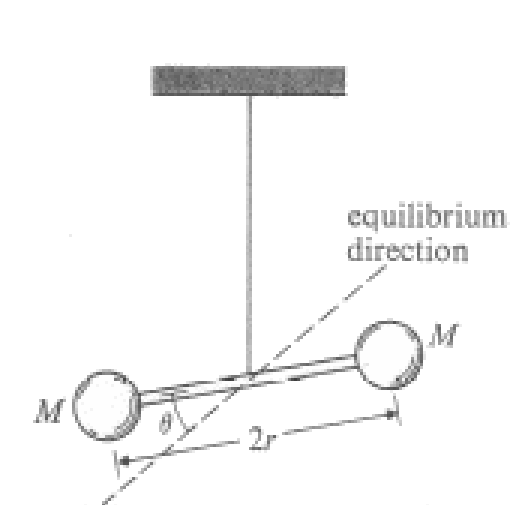
\includegraphics[width=0.8\textwidth]{fotos/dumbell.png}
\end{wrapfigure}
A dumbbell is hung from a thin wire of ignorable mass attached at the midpoint. If the wire twists by angle $\theta$ from equilibrium, it accrues potential energy $U(\theta)=\frac12 C\theta^2$, where $C$ is a positive constant. From equilibrium, the dumbbell is rotated through angle $\theta_0$ and then released. Use the energy method to find the differential equation governing the oscillations of the dumbbell and from it, find the frequency of oscillations. Ignore friction. Ignore the mass of the rod that connects the two spherical masses; take each as a point mass. Show all steps of the logic.\\

\noindent Specifically use the (full) energy method (not the “quick energy method”). Clearly show all steps of the logic, including (where needed) English sentence justification. The masses are each $M$, their center-to-center separation is $2r$. The kinetic energy involves the moment of inertia of the two masses with their given (unchanging) separation.}

  \noindent For this exercise, I will denotate $\omega=\dot{\theta}$ as the angular velocity and $f$ as the frequency of the oscilation so as not to confuse them. The full energy method involves obtaining an expression for the energy and then derivating with respect to time. Then the energy of the system is:
  \[E=K+U=\dfrac12 I\omega^2+\dfrac12 C\theta^2 = \dfrac12 I\dot{\theta}^2+\dfrac12 C\theta^2\]
  \[\dfrac{dE}{dt}=0\Longleftrightarrow I\dot{\theta}\ddot{\theta}+C\theta\dot{\theta}=0\Longleftrightarrow I\ddot{\theta}+C\theta=0 \Longleftrightarrow \ddot{\theta}+\dfrac{C}{I}\theta=0\]
  \[f=\sqrt{\dfrac{C}{I}}=\sqrt{\dfrac{C}{2Mr^2}}\]
  \noindent Assuming that that $I=2Mr^2$
  \clearpage
%%%%%%%%%%%%%%%%%%%%%%%%%%%%%%%%%%%%%%%%%%%%%%%%%%%%%%%%%%%%%%%%%%%%%%%%%%%%%
\pregunta{Derive the governing differential equation for the charge oscillations of an LC circuit by the energy method. Ignore resistance. Use the “full energy method.” Show all necessary steps of the derivation.}

  \noindent As on the last exercise, we will write the energy of the system, then derive respect to the time and get the ode.
  \[E=U_C+U_L=\dfrac12 CV^2+\dfrac12 LI^2=\dfrac12 C\left(\dfrac{Q}{C}\right)^2+\dfrac12 L\left(\dfrac{dQ}{dt}\right)^2\Longleftrightarrow E=\dfrac12 \dfrac{Q^2}{C}+\dfrac12 L\left(\dfrac{dQ}{dt}\right)^2\]
  \[\dfrac{dE}{dt}=0\Longleftrightarrow \dfrac{1}{C}\dot{Q}Q + L\dot{Q}\ddot{Q}=0\Longleftrightarrow \dfrac{Q}{C} +L\ddot{Q}=0\Longleftrightarrow \boxed{\dfrac{1}{LC}Q+\ddot{Q}=0}\]
%%%%%%%%%%%%%%%%%%%%%%%%%%%%%%%%%%%%%%%%%%%%%%%%%%%%%%%%%%%%%%%%%%%%%%%%%%%%%
\pregunta{
\begin{wrapfigure}[7]{r}{0.18\textwidth}
  \vspace{-0.65cm}
  \centering
  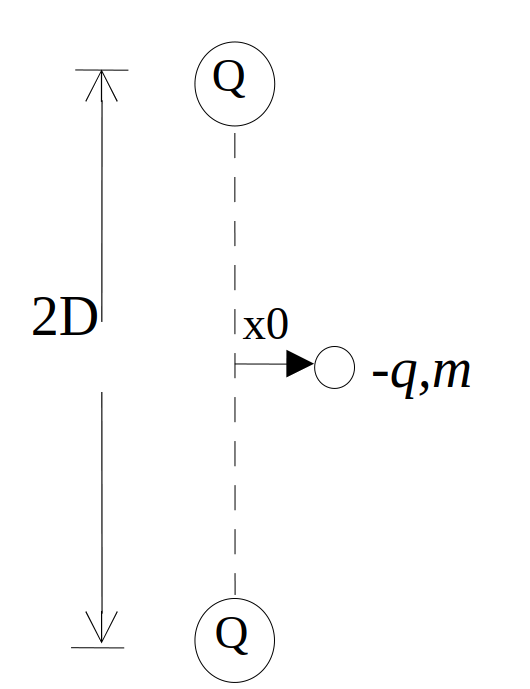
\includegraphics[width=0.95\textwidth]{fotos/charges.png}
\end{wrapfigure}

Two identical positive charges $Q$ are held in place at distance $2D$ apart. A small mass $m$ carrying negative charge $-q$ is released from rest at distance $x_0$ from the point midway between the positive charges as shown. $x_0 << D$.

\vspace{0.5cm}Ignoring $x_0$ compared to $D$, find the appropiate frequency of the resulting oscillations of $q$. "Zero" is not a good enough answer. The exercise is to show all steps of the correct derivation of the result. You need not rederive basic results from first year physics.\\

\vspace{0.3cm}\textit{\underline{Hints}: Use Newton's second law to derive the governing differential equation (“g.d.e.”). Remember that a return (to equilibrium) force has a minus sign. In the resulting g.d.e., express $\sin(\theta)$ in terms of $x$ and $D$.\\
\underline{Answer}: $\omega^2\approx \dfrac{qQ}{2\pi\varepsilon_0 m D^3}$}}

  \noindent The electric force between two charges is defined by Coulomb's Law, in modulus:
  \[F_e = \dfrac{kqQ}{r^2}\]
  \noindent The electric force in our system will be doubled because of the two charges. We can decompose the forces into the axis and discard the vertical component thanks to the symmetry of the problem. Since $v(0)=0$ and $x(0)=x_0<<D$ we can use the small angle approximation in this problem. Moreover, from the figure we can see that $sin(\theta)=\theta=\nicefrac{x}{D}$. Then:
  \[F = -\dfrac{2kqQ}{\sqrt{x_0^2+D^2}}\sin(\theta) = -\dfrac{qQ}{2\pi\varepsilon_0}\dfrac{x}{D\sqrt{x_0^2+D^2}}=m\ddot{x} \]
  \noindent As $x_0 << D$, then:
  \[\sqrt{x_0^2+D^2}\approx D^2 \Longleftrightarrow \ddot{x}=-\dfrac{qQ}{2\pi\varepsilon_0 mD^2} x \Longleftrightarrow \boxed{\omega^2\approx\dfrac{qQ}{2\pi\varepsilon_0 mD^2}}\]

\clearpage
%%%%%%%%%%%%%%%%%%%%%%%%%%%%%%%%%%%%%%%%%%%%%%%%%%%%%%%%%%%%%%%%%%%%%%%%%%%%%
\pregunta{Complete the analysis of the worked example shown below. Use either version of the energy method to find the frequency of oscillations. Assume that the center of mass is stationary.\\
\begin{center}
  \textbf{Partially Worked Example:}\\
  \textbf{Oscillation Model For Diatomic Molecule With Unequal Ion Masses: }
\end{center}
\begin{wrapfigure}[4]{r}{0.42\textwidth}
  \vspace{-0.7cm}
  \centering
  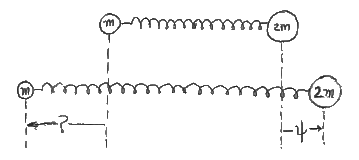
\includegraphics[width=0.93\textwidth]{fotos/example.png}
\end{wrapfigure}

Suppose the ion masses are $m$ and $2m$. Find the frequency of the "breathing mode".\vspace{0.6cm}\\
\textit{\underline{Solution}: The figure shows the equilibrium and arbitrary configurations for the breathing mode.}\\

\noindent Let's first use the method of 'physical meaning of $\omega^2$'. We work in the CM frame, so the CM itself is stationary. I'll outline ome steps for you:
\begin{enumerate}[label=\alph*.]
  \item If $\psi$ represents the displacement of $2m$ from equilibrium, what must the simultaneous displacement of $m$ (labeled '?' in figure) be?
  \item Based on your anwser to part \textit{a}, what do you expect the frequency of 'breathing oscillation' of the molecule to be?
\end{enumerate}
\underline{\textit{Answers}}:
\begin{enumerate}[label=\alph*.]
  \item \textit{To keep the center of mass stationary, if mass $2m$ moves a distance $\psi$ from equilibrium, then mass $m$ muss move a distance $2\psi$ (in the opposite direction).}
  \item \textit{Note that a stretched spring exerts an equal force at each of its ends. Now, in the 'arbitrary configuration' shown, the total stretch of the spring is $3\psi$ (compared to the equilibrium configuration). Thus, the force on mass $2m$ is $-3k\psi$; hence the equation of motion of $2m$ is $2m\ddot{\psi}=-3k\psi$, which means thatm mass $2m$ should oscillate in simple harmonic motion with frequency $\omega^2=\nicefrac{3k}{2m}$.}
\end{enumerate}
\noindent Now consider mass $m$. It must oscillate in simple harmonic motion at the same frequency as does mass $2m$; otherwise, the CM would accelerate. The force on it is also $-3k\psi$ and its displacement is $2\psi$, so its equation of m otion is $m(2\ddot{\psi})=-3k\psi$, which confirms that $m$ oscillates in simple harmonic motion. This oscillation is $180^\circ$ out of phase with that of $2m$.\\

\noindent Use the energy method to find the frequency of the breathing mode for the 'molecule'.\\
\noindent \textit{\underline{Solution}: The first step is to write the total energy in the arbitrary configuration:
\[E=\dfrac12 m(2\dot{\psi})^2+\dfrac12(2m)(\dot{\psi})^2+\dfrac12 k(3\psi)^2\]} }

  \noindent To continue on the worked example, we will derivate the energy function with respect to time. As this function is a constant, then its temporal derivative will be zero:
  \[\dfrac{dE}{dt}=0\Longleftrightarrow \dfrac{d}{dt}\left(2m\dot{\psi}^2+m\dot{\psi}^2+\dfrac92 k\psi^2\right)=\dfrac{d}{dt}\left(3m\dot{\psi}^2+\dfrac92 k\psi^2\right)=0\Longleftrightarrow\]
  \[\Longleftrightarrow 6m\dot{\psi}\ddot{\psi}+9k\psi\dot{\psi}=0\Longleftrightarrow 6m\ddot{\psi}+9k\psi = \ddot{\psi}+\dfrac{9k}{6m}\psi=0\Longleftrightarrow \boxed{\omega^2=\dfrac{3k}{2m}}\]
%%%%%%%%%%%%%%%%%%%%%%%%%%%%%%%%%%%%%%%%%%%%%%%%%%%%%%%%%%%%%%%%%%%%%%%%%%%%%
\pregunta{Using the spring model we've been working with, find the oscillation frequency for a 'diatomic molecule' in which the ions have unequal masses $m$ and $M$ respectively:
\begin{enumerate}[label=\alph*.]
  \item First use the “method of physical meaning of $\omega^2$ we used in Worked Example. Make sure you obtain the same frequency applying the method to each of the masses.
  \item Then use the formalism of the energy method.
\end{enumerate}
\textit{\underline{Answer}: $M\ddot{\psi}=-\left(1+\frac{M}{m}\right)k\psi$}}
\subsubsection*{Physical meaning of $\omega^2$ method}
  \noindent As on the previous example, the displacement from equilibrium must mantain the center of mass equal. Then, if the displacement from mass $M$ is called $\psi$, the displacement of mass $m$ that mantains the center of mass stationary is a distance $\psi\nicefrac{M}{m}$ in the opposite direction. Then, the total stretch is $\psi(1+\nicefrac{M}{m})$.
  \noindent Because of that, the force on both of the masses will be equal (so as not to accelerate the CM), but the equation for each one will be: $M\ddot{\psi}=-\psi k(1+\nicefrac{M}{m})\ \ $ and $\ \ m(\frac{M}{m}\ddot{\psi})=-\psi k(1+\nicefrac{M}{m})$ which will result in the same ode (and thus the same frequency but at $180^\circ$ out of phase from each other): 
  \[\boxed{M\ddot{\psi}=-(1+\nicefrac{M}{m})k\psi} \Longleftrightarrow \omega=\sqrt{\left(\dfrac{1}{M}+\dfrac{1}{m}\right)k}\Longleftrightarrow\boxed{\omega=\sqrt{\mu k}}\]
\subsubsection*{Energy method}
  \noindent As on the example, first of all we have to work out an expression for the total energy:
  \[E=K_m+K_M+U_s=\dfrac12 m\left(\dfrac{M}{m}\dot{\psi}\right)^2 + \dfrac12 M(\dot{\psi})^2 + \dfrac12 k \left(\left(1+\dfrac{M}{m}\right)\psi\right)^2\]
  \noindent Now we derivate with respect to time and equal it to zero, because the energy is constant.
  \[\dfrac{dE}{dt}=0\Longleftrightarrow \dfrac{d}{dt}\left(\dfrac12 \dfrac{M^2}{m}\dot{\psi}^2+\dfrac12 M\dot{\psi}^2+\dfrac{k}{2}\left(1+\dfrac{M}{m}\right)^2\psi^2\right)=\dfrac{M^2}{m}\dot{\psi}\ddot{\psi}+M\dot{\psi}\ddot{\psi}+k\left(1+\dfrac{M}{m}\right)^2\psi\dot{\psi}=0\Longleftrightarrow\]
  \[\Longleftrightarrow M\left(1+\dfrac{M}{m}\right)\ddot{\psi}+k\left(1+\dfrac{M}{m}\right)^2\psi\Longleftrightarrow \boxed{M\ddot{\psi}+k\left(1+\dfrac{M}{m}\right)\psi=0} \Longleftrightarrow \boxed{\omega=\sqrt{\mu k}}\]
  \noindent Which is the same result we got with the previous method.

\end{document}
